\chapter{Commercialization Plan}

\section{Introduction}

The RSL Rover is a robotic vehicle prototype designed to aid in the process of post fire investigation. The RSL Rover design is built around integrating individual subsystems under the industry standard Robotic Operating System (ROS) in order to create a vehicle capable of driving fire fighters to areas affected by forest fires, proceeding unmanned into said area, visually scanning the area, creating 3D visual maps using LIDAR technology and GPS location, gathering data on various dangerous gasses, the temperature, air particulates, and smoke, storing the data for future dissemination, and presenting important data live to users on an interface that is accessible and easy to understand. While this vehicle is a prototype built around the technology available to the RSL at Santa Clara University, our final design would integrate our modular environmental sensing and mapping subsystems to a modified drive-by-wire vehicle such as a Ford F-150 so that our product can be useful in a variety of disaster situations. We would seek to market our design to both government funded and privately funded forest fire fighting organizations. Though forest fire fighting services already have a process they go through during the stages of post-fire investigation, these processes are dangerous for the fire fighters who enter in to scan the area before any other kinds of ground-level assessments have been made. Though currently many fire fighting agencies are purchasing UAV's for robotic assistance in post fire investigation, these platforms have many disadvantages in comparison to the RSL Rover.

\section{Goals and Objectives}

Our company's main objective is to keep disaster responders out of harm's way. Responders will use our unmanned, modular vehicle to assess the environment that has been affected by a disaster. Our vehicles are driven remotely and collect a variety of meaningful data and our user interface elegantly displays this data to the operators, who are located far from the disaster zone at a safe distance. With this data, operators can make educated decisions regarding the subsequent steps that must be taken in order to recover the affected area. Our goal is to ensure that responders are not subjecting themselves to any environmental hazards during this disaster response process. 

Our vision for the commercialization of our product is to provide unmanned and modular disaster response vehicles to a variety of public and private disaster response and recovery departments. To do this, we will work closely with these departments to offer useful vehicles that can be used to assess environments that have been affected by various disasters. Our company will develop these vehicles with the proper environmental sensors and user interface for the specific needs of the customer in question. For example, our prototype was developed with fire response in mind (see Chapter 3 for a more detailed description of our prototype). 

\section{Description}

The RSL Rover is unlike any product currently on the market. It is a modular drive-by-wire vehicle designed to serve emergency responders in all types of natural disasters and emergency situations. The drive-by-wire system allows emergency personel to operate the vehicle at a safe distance while still being able to collect relevant ground level information about an area. The vehicle is not limited to drive-by-wire, though; it is also capable of being controlled manually so that it can be driven to the command center rather than being towed there. This also means that the vehicle will not only be limited to remote operation missions, it could also be utilized in scenarios where remote driving is not necessary.\newline

\begin{figure}[h!]
	\begin{center}
		\includegraphics[width=0.6\linewidth]{FireRover.JPG}
		\caption{The RSL Rover monitoring air quality around a controlled burn in California}
		\label{fig:FireRover}
	\end{center}
\end{figure}

Current modular packages that could be outfitted onto the vehicle include a smoke and fire-gas detection package useful in forest fire investigations and a flammable and toxic gas detection package for urban and suburban natural disaster response. Figure \ref{fig:FireRover} shows one capability of the vehicle where it is monitoring air quality during a controlled burn in the central valley of California. Additionally, the vehicle is capable of generating 3-dimensional maps of an environment so that emergency personnel can have the most information to make informed decisions on response plans. The platform for a versatile, multi-function vehicle is there with the RSL Rover; it is up to fire departments and emergency services to discover the many functions the RSL Rover has to offer.

\section{Potential Markets}

The RSL Rover is meant to be marketed towards forest fire fighting agencies. These agencies range from the United States Forest Service, which currently has 750 locations, hires over 30,000 employees, of which a third are fire fighters, and has an annual budget of over \$5.5 billion, to private forestry services, such as the National Wildfire Suppression Association who represent over 150 private wildfire services that contract out work on an as-needed basis to fight fires. Both of these styles of forest fire fighting rely on the bravery of fire fighters to analyze areas affected by forest fires, and thus our product could provide the capabilities to remove people from harms way during the period of post fire investigation.

We were lucky enough to talk to Lieutenant Firefighter Perez from the Santa Clara Fire Department, who told us that his department is given an annual budget of around one-million dollars for new equipment. While budgets vary from area to area, it can be assumed that fire fighting agencies are given high amounts of money for the purchasing of equipment that could be spent on our vehicle. As many fire fighting agencies are considering drone technologies for fire reconnaissance, we believe that this market is one that we can tap into, as our vehicle not only provides reconnaissance, but also many levels of useful data to fire fighters. 

\section{Competition}

Many all-terrain, unmanned vehicles on the market are for military contracts exclusively. However, Northrop Grumman and Argo Robotics both have products that fit the category of an unmanned, all-terrain vehicle that can be equipped with sensor packages for non-military purposes. Some of the specs for these products can be found in Table 2.1. These are the Argo J5 Mobility Platform at thirty-nine-thousand dollars, the Northrop Grumman Andros F6, and the Northrop Grumman Wheelbarrow Mk9. Prices for the two later vehicles are not available without a direct quote. 

\begin{table}[H]
	\begin{adjustwidth}{-.5in}{-.5in}
		\centering
		\begin{tabular}{c|c|c|c|c|c}
			Product & Height(m) & Width(m) & Length(m) & Sensor Packages & Features\\\hline
			J5 Mobility Platform & 0.83 & 1.38 & 1.52 & 1 Camera Mount & Amphibious\\
			Andros F6 & 1.486 & 0.445 & 1.32 & 5 Cameras & Extendable Arm \\
			Wheelbarrow Mk9 & 1.24 & 0.63 & 1.24 & Up to 10 Cameras & Extendable Arm\\
		\end{tabular}
		\caption{\label{tab:current} Current Product Comparison}
	\end{adjustwidth}
\end{table}

While these products that are on the market are the most similar to the product we wish to produce, the issues we wish to address are not solved by these rovers. Both of Northrop Grumman's rovers do not have the housing needed for sensor packages necessary to respond to forest fires. The Argo rover also does not house the necessary data packages, and while it is amphibious, we have concluded through our research and customer interactions that the sensor housing is more important.

Other Aerial Drones are also in the market for unmanned vehicles capable of relaying data such as thermal imaging and video back to the user. Two such products are the Elimco UAV-E300 and the Sensefly's EBee. Both of these products have the capabilities necessary to map and relay usable data, and are marketed as disaster response vehicles. However, there are some inherent weaknesses to their aerial nature. Images provided by Aerial vehicles can oftentimes be unusable as smoke can sit on top of the canopy of a forest, especially in the mornings. They also can only provide overhead data, and may not be able to map certain elements disaster responders could need, such as air quality at ground level or mapping paths that are safe. Our vehicle seeks to get under this layer of smoke to provide data from the ground level.


\section{Sales and Marketing Strategy}

In order to market and sell our product, we would need to target national and international disaster response departments and make our product visible within the department communities. 

To make our product visible and generate interest, we must get communities involved in the effort to keep disaster responders out of harm's way. We can create a series of disaster response community training efforts. For example, we could offer members of a community courses where they can learn what to do in the event of an earthquake or fire where we would also educate them on the sort of dangers disaster responders face in their daily lives. We can also make efforts to establish a relationship with local media outlets. For example, local news channels can highlight our product during a segment on innovation in robotics or on disaster response education. Through strategies such as these, we will be able to market our product by establishing a presence within the communities our product can help in the event of a disaster. This presence will encourage disaster departments to adopt our technology. 

When advertising our product, our company's main goal is to emphasize how these vehicles can save the lives of the brave disaster responders who serve to protect our communities in the event of an earthquake, fire, etc. Our vehicles allow the responders to assess the environment that has been affected by a disaster from a safe distance. With our product, these responders will not have to subject themselves to dangers such as unstable structures or toxic gases in the air. Our company should convey this message clearly through our advertising efforts so that potential customers can immediately recognize the great value of our product. 

In order to sell our vehicles, we would have to employ company representatives in multiple states and countries. These representatives will meet with the department leads to determine what their specific department needs are and whether our company can meet those needs. If an agreement is made and the department purchases one or more vehicle(s), the vehicle will be hauled from one of our factories to the department location. A minimal amount of training for these disaster responders would be included. The regional/statewide/countrywide company representative will also be responsible for holding a training workshop for the responders. 

\section{Manufacturing Plan}

Manufacturing facilities have been minimized by using the existing platform of Ford F-150 pickup trucks as the base for the RSL Rover. The trucks will be outfitted in our warehouse by trained technicians. Manufacturing the RSL Rover at the same location where it is designed will allow the engineers to have the oversight necessary to ensure manufacturing goes according to plan. It also makes it possible to quickly implement design changes as needed. This will require the lease of a warehouse facility with welding equipment, 3-phase power, hydraulic hoists, and a large footprint. The initial process of training technicians and outfitting the warehouse will be the most time consuming part of the process. Once the initial setup is complete, the vehicles will take approximately 200 hours to manufacture and test. This initial phase will be costly and likely require one million dollars, including the upfront research and development costs.

To offset these large costs, the production goal will be 100 to 200 vehicles per year. According to the cost estimates outlined in the following section, this will net five million to ten million dollars in revenue annually. As demand increases, more warehouses will be opened throughout the nation and potentially globally if the global market is receptive to the vehicle.

Manufacturing will take place in four phases. The first phase of the process will be outfitting the vehicle with the drive-by-wire system that is the heart of the vehicle's functionality. The importance of this system is reinforced by the next phase; phase two of manufacturing is the rigorous testing of the drive-by-wire system. After the drive-by-wire system is installed and tested, the Lidar and cameras will be outfitted to the vehicle to provide vision for the operators and analysts. The final stage of production is outfitting the vehicle with the selected modular sensing packages. There are multiple packages to choose from that allow functionality for different types of disasters.

\section{Product Cost and Price}

The vehicle will be built upon the existing platform of a Ford F-150 truck in an effort to minimize construction costs and maximize utility for fire fighters. The breakdowns for manufacturing costs are listed in tables \ref{table:ComponentCosts} and \ref{table:LaborCost} and the cost of producing a single vehicle at any volume is listed in table \ref{table:VehicleCost}.

\begin{table}[h!]
	\begin{center}
		\begin{tabular}{| l | c |}
			\hline
			\textbf{Component} & \textbf{Price} \\ \hline
			Drive-By-Wire Outfitting & \$5,000 \\ \hline
			F-150 vehicle platform & \$31,000 \\ \hline
			Modular Sensing Package(s) & \$1,000 ea \\ \hline
			Velodyne Puck Lidar & \$7,999 \\ \hline \hline
			\textbf{Total Component Cost} & \$44,999+ \\ \hline
		\end{tabular}
	\end{center}
	\caption{Component cost breakdown}
	\label{table:ComponentCosts}
\end{table}

\begin{table}[h!]
	\begin{center}
		\begin{tabular}{| l | c |}
			\hline
			Labor Cost/hr & \$20 \\ \hline
			Labor Hours/vehicle & 250 \\ \hline \hline
			\textbf{Labor Cost per Vehicle} & \$5,000 \\ \hline
		\end{tabular}
	\end{center}
	\caption{Labor breakdown}
	\label{table:LaborCost}
\end{table}

\begin{table}[h!]
	\begin{center}
		\begin{tabular}{| l | c |}
			\hline
			Component Cost per Vehicle & \$44,999 \\ \hline
			Labor Cost per Vehicle & \$5,000 \\ \hline \hline
			\textbf{Cost per Vehicle} & \$49,999 \\ \hline
		\end{tabular}
	\end{center}
	\caption{Cost per Vehicle}
	\label{table:VehicleCost}
\end{table}

The vehicle will be priced at \$100,000 base with additional modular packages available for purchase and integration. The profits associated with the sale will fund the development costs of the vehicle as well as future research and development of modular accessories.

There are no direct competitors to the RSL Rover but the available budgets of departments should be considered. A Typical, mid-sized department has a million dollar annual budget for equipment. This means that it would be relatively easy for fire departments to add RSL Rovers to their fleets. Even small departments will be able to afford them and large departments will be able to purchase several per year. According to the United States Fire Administration, there are over 25,000 registered fire departments in the U.S. Therefore, it is reasonable to predict 100 vehicle sales annually. This would allow for significant reasearch efforts and cover the initial development costs in just one year.

\section{Service and Warranties}

Since we plan on using existing vehicles (such as a Ford F-150) as a platform to apply our technology to, warranties must be handled solely by our company. We would be modifying the existing vehicle to a degree that would potentially void the car warranty. This potential loss of warranty is caused by the chance that any modifications we make to the vehicle can be the reason why the vehicle fails. The vehicle mechanical components should last roughly as long as the vehicle manufacturer claims they should last. However, we cannot predict the type of wear and tear the vehicle will experience with the subsystems we introduce. 

If our product were to fail, it would be the company's responsibility to diagnose the issue and replace the necessary parts. Since our product includes complicated electrical subsystems and modified driving components we cannot expect on-site or local mechanics to know how to fix them. In some cases, like in highly populated cities, disaster response departments have their own mechanic. Or, in smaller cities and towns, these departments have local shops that they turn to when their equipment requires maintenance.  Our company could introduce a special contract with automotive parts retailers as well as automotive repair shops in order to quickly and locally rectify the vehicle's small mechanical issues  for the departments. For the more complicated subsystems and driving components that we introduce, we would need to have a series of specially trained technicians that can travel to the locations of disaster departments and repair the vehicles. We could require a yearly maintenance fee from the disaster departments in order to cover these costs. 

\section{Financial Plan and ROI}

As was previously mentioned in our Cost and Price section, our vehicles when manufactured should have a cost of around \$49,999, and we feel that due to the capability of our vehicle to protect human lives, the research and development of robotic solutions to the problem, as well as the amount of skilled labor being put into combining the multiple subsystems into a usable and applicable device our price is set at \$100,000. In order to estimate overhead, our team looked for warehouse space to establish as a workshop through LoopNet, a website dedicated to renting commercial real estate. We established a relative average of around \$15 per square foot per year. Thinking that we would need at least 500 square feet for production of 20 or less vehicles in a year, while moving up 1000 square feet for production of 50 or more vehicles. Our plan would be to sell 5 vehicles in our first year to initial buyers, then expanding our market every year based on our profits we acquire. We also had an extra \$2000 in overhead for the first year in case of extra expenses. In order to cover the costs of the first year, we would need an investment of around \$30,000 (or perhaps a loan if we are desperate), followed by continuing to find investors for the future two years. Our goal is then to work up to selling 100 units per year. The Return on investment and Financial plan is shown in the figure below.

\begin{figure}[h!]
	\begin{center}
		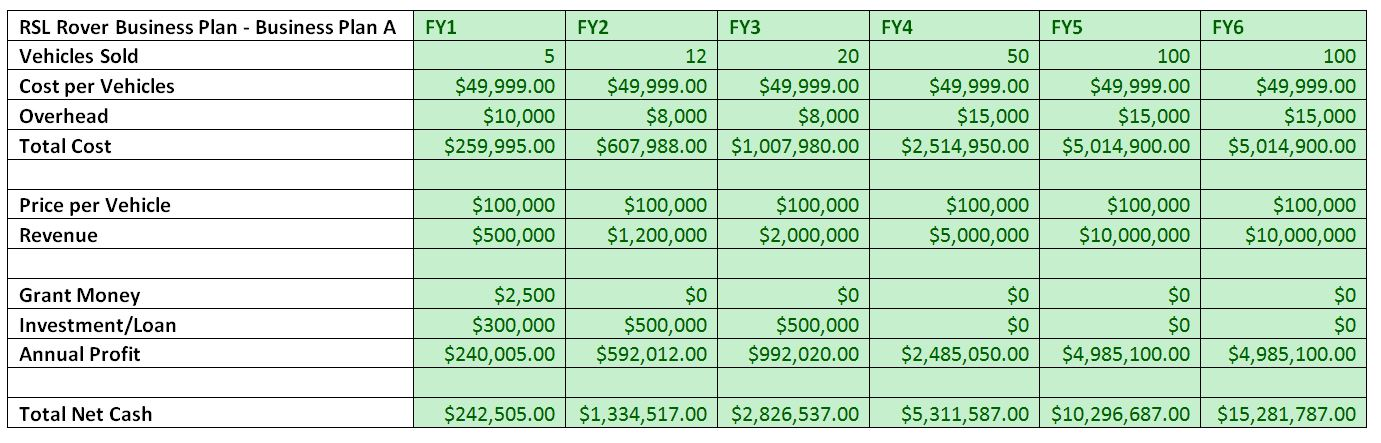
\includegraphics[scale=0.5]{RSL_Rover_Business_plan.JPG}
		\caption{Excel table showing Team RSL Rover's estimated financial plan and return of investment}
		\label{fig:FinPlan}
	\end{center}
\end{figure}